\documentclass[10pt,fleqn,a4paper]{article}

\usepackage[utf8]{inputenc}
\usepackage[T2A]{fontenc}
\usepackage{fullpage}
\usepackage[russian]{babel}
\usepackage{amsthm,amsmath,amsfonts,amssymb}
\usepackage{bussproofs}
\usepackage{listings}
\usepackage{multirow}
\usepackage{xcolor}
\usepackage{tikz}
\usepackage{graphicx}
\usepackage{caption}
\usepackage{float}
\usepackage{subcaption} 
\usepackage{hyperref}
\DeclareGraphicsExtensions{.pdf,.png,.jpg}
\usepackage{indentfirst}
\graphicspath{{img/}}
\usetikzlibrary{graphs}

\newtheorem{problem}{Задача}

\newenvironment{solution}
  {\renewcommand\qedsymbol{$\blacksquare$}\begin{proof}[Решение]}
  {\end{proof}}
  
\newtheorem*{definition}{Определение}

%\newcommand{\mod}{\texttt{mod}}
\renewcommand{\H}{\mathcal{H}}
\newcommand{\F}{\mathbb{F}}
\newcommand{\Z}{\mathbb{Z}}
\newcommand{\N}{\mathbb{N}}

\newcommand{\lcm}{\texttt{lcm}}
\newcommand{\Prb}[1]{\underset{#1}{\textbf{Pr}}}
\newcommand{\Prbb}[2]{\underset{#1}{\textbf{Pr}}\left[ \; #2 \;\right]}
\newcommand{\Ex}[1]{\underset{#1}{\textbf{E}}}
\newcommand{\exceptgroup}[1]{\textit{(кроме группы #1)}}
\newcommand{\onlygroup}[1]{\textit{(только группа #1)}}

\renewcommand{\O}{\mathcal{O}}
\renewcommand{\t}[1]{\texttt{#1}}  

\begin{document}

  \definecolor{dkgreen}{rgb}{0,0.6,0}
  \definecolor{gray}{rgb}{0.5,0.5,0.5}
  \definecolor{mauve}{rgb}{0.58,0,0.82}  

  \newcommand{\problemset}[1]{
    
    \begin{center}
      \Large #1
    \end{center}
  }

  \lstset{ %
    language=C++,                % the language of the code
    basicstyle=\footnotesize,           % the size of the fonts that are used for the code
    numbers=left,                   % where to put the line-numbers
    numberstyle=\tiny\color{gray},  % the style that is used for the line-numbers
    stepnumber=1,                   % the step between two line-numbers. If it's 1, each line 
                                    % will be numbered
    numbersep=5pt,                  % how far the line-numbers are from the code
    backgroundcolor=\color{white},      % choose the background color. You must add \usepackage{color}
    showspaces=false,               % show spaces adding particular underscores
    showstringspaces=false,         % underline spaces within strings
    showtabs=true,                 % show tabs within strings adding particular underscores
    frame=single,                   % adds a frame around the code
    rulecolor=\color{black!10},        % if not set, the frame-color may be changed on line-breaks within not-black text (e.g. comments (green here))
    tabsize=2,                      % sets default tabsize to 2 spaces
    captionpos=b,                   % sets the caption-position to bottom
    breaklines=true,                % sets automatic line breaking
    breakatwhitespace=false,        % sets if automatic breaks should only happen at whitespace
    title=\lstname,                   % show the filename of files included with \lstinputlisting;
                                    % also try caption instead of title
    keywordstyle=\color{blue},          % keyword style
    commentstyle=\color{dkgreen},       % comment style
    stringstyle=\color{mauve},        % string literal style
    escapeinside={\%*}{*)},            % if you want to add LaTeX within your code
    morekeywords={done, to},              % if you want to add more keywords to the set
  %  deletekeywords={...}              % if you want to delete keywords from the given language
  }

  \begin{tabbing}
\hspace{11cm} \= Студент: \= Максим Васильев (285800)\\
  \> Группа: \>  M4140 \\
  \> Дата: \> \today
\end{tabbing}
\hrule
\vspace{1cm}


  % \section{Многозначные логики}
\begin{enumerate}
  \item (3 балла) В какой из многозначных логик, рассмотренных выше, истинны все пропозициональные тавтологии? Обоснуйте ваш ответ.
  \begin{solution}
    В логике Приста истинными считаются как $T$, так и $I$, поэтому можно сказать, что именно в этой логике истинны все пропозициональные тавтологии, потому что они строятся таким образом, чтобы никогда не получалось $F$. Если будут получаться $T$ или $I$, то нас это будет устраивать, раз $I$ считается истинным.
  \end{solution}
  \item Определите связку $\leftrightarrow$ для следующих логик:
  \begin{enumerate}
    \item (1 балл) сильная логика Клини, таблица истинности
    \begin{solution}
      По определению $A \leftrightarrow B = (A \rightarrow B) \land (B \rightarrow A)$.
      \begin{displaymath}
      \begin{array}{c c|c|c|c}
        A & B & A \rightarrow B & B \rightarrow A & A \leftrightarrow B\\
        \hline
        T & T & T & T & T\\
        T & I & I & T & I\\
        T & F & F & T & F\\
        I & T & T & I & I\\
        I & I & I & I & I\\
        I & F & I & T & I\\
        F & T & T & F & F\\
        F & I & T & I & I\\
        F & F & T & T & T
      \end{array}
      \end{displaymath}
    \end{solution}
    \item (1 балл) слабая логика Клини, таблица истинности
    \begin{solution}
      \begin{displaymath}
      \begin{array}{c c|c|c|c}
        A & B & A \rightarrow B & B \rightarrow A & A \leftrightarrow B\\
        \hline
        T & T & T & T & T\\
        T & I & I & I & I\\
        T & F & F & T & F\\
        I & T & I & I & I\\
        I & I & I & I & I\\
        I & F & I & I & I\\
        F & T & T & F & F\\
        F & I & I & I & I\\
        F & F & T & T & T
      \end{array}
      \end{displaymath}
    \end{solution}
    \item (1 балл) логика Приста, таблица истинности
    \begin{solution}
      \begin{displaymath}
      \begin{array}{c c|c|c|c}
        A & B & A \rightarrow B & B \rightarrow A & A \leftrightarrow B\\
        \hline
        T & T & T & T & T\\
        T & I & I & T & I\\
        T & F & F & T & F\\
        I & T & T & I & I\\
        I & I & I & I & I\\
        I & F & I & T & I\\
        F & T & T & F & F\\
        F & I & T & I & I\\
        F & F & T & T & T
      \end{array}
      \end{displaymath}
    \end{solution}
    \item (1 балл) логика Гёделя, кусочно-заданная функция
    \begin{solution}
      Возможные значения:
      \begin{equation}
        A_i = 0, \frac{1}{k-1}, \frac{2}{k-1}, \dots, \frac{k-2}{k-1}, 1.
      \end{equation}
      При проходе по множеству в сторону увеличения $A_i$ будем получать случай $A_i\leq A_{i+1}$, поэтому функция $A\rightarrow B$ будет во всех точках равна 1.
      \begin{equation}
        A\rightarrow B = 1.
      \end{equation}
      В случае $B\rightarrow A$ случаи в импликации будут другими, будет выбираться значения $B$, поэтому функция будет следующей:
      \begin{equation}
        B\rightarrow A =
        \begin{cases}
          0, & [0, \frac{1}{k-1}] \\
          \frac{1}{k-1}, & (\frac{1}{k-1}, \frac{2}{k-1}] \\
          \dots \\
          \frac{k-2}{k-1}, & (\frac{k-3}{k-1}, \frac{k-2}{k-1}] \\
          1, & (\frac{k-2}{k-1}, 1]
        \end{cases}
      \end{equation}
      Так как конъюнкция определяется как минимум, то итоговая функция будет аналогичной:
      \begin{equation}
        B\leftrightarrow A =
        \begin{cases}
          0, & [0, \frac{1}{k-1}] \\
          \frac{1}{k-1}, & (\frac{1}{k-1}, \frac{2}{k-1}] \\
          \dots \\
          \frac{k-2}{k-1}, & (\frac{k-3}{k-1}, \frac{k-2}{k-1}] \\
          1, & (\frac{k-2}{k-1}, 1]
        \end{cases}
      \end{equation}
    \end{solution}
  \end{enumerate}
  \item (3 балла) Рассмотрим функцию голосования $maj(x_1, ..., x_n)$. Она обращается в единицу, когда среди поданных на вход значений, единиц не меньше, чем нулей. В остальных случаях она обращается в ноль. Выпишите полином Жегалкина методом неопределённых коэффициентов для функции $maj(x_1, x_2, x_3)$.
  \begin{solution}
    Составим таблицу истинности на основе условия:
    \begin{displaymath}
      \begin{array}{c c|c|c}
        x_1 & x_2 & x_3 & maj\\
        \hline
        0 & 0 & 0 & 0\\
        0 & 0 & 1 & 0\\
        0 & 1 & 0 & 0\\
        0 & 1 & 1 & 1\\
        1 & 0 & 0 & 0\\
        1 & 0 & 1 & 1\\
        1 & 1 & 0 & 1\\
        1 & 1 & 1 & 1
      \end{array}
      \end{displaymath}
    Выпишем формулу в общем виде для трех переменных:
    \begin{equation}
      maj(x_1,x_2,x_3)=a_0 \oplus a_1x_1 \oplus a_2x_2 \oplus a_3x_3 \oplus a_{12}x_1x_2 \oplus a_{13}x_1x_3 \oplus a_{23}x_2x_3 \oplus a_{123}x_1x_2x_3.
    \end{equation}
    Действуем по алгоритму в порядке увеличения числа единиц:
    \begin{eqnarray}
      0=maj(0,0,0)=a_0 \Rightarrow a_0 = 0 \\
      0=maj(0,0,1)=a_3 \Rightarrow a_3 = 0 \\
      0=maj(0,1,0)=a_2 \Rightarrow a_2 = 0 \\
      0=maj(1,0,0)=a_1 \Rightarrow a_1 = 0 \\
      1=maj(0,1,1)=a_{23} \Rightarrow a_{23} = 1 \\
      1=maj(1,0,1)=a_{13} \Rightarrow a_{13} = 1 \\
      1=maj(1,1,0)=a_{12} \Rightarrow a_{12} = 1 \\
      1=maj(1,1,1)=1\oplus 1\oplus 1\oplus a_{123} \Rightarrow a_{123} = 0
    \end{eqnarray}
    Отсюда получается, что полином Жегалкина для $maj$ следующий:
    
    \textbf{Ответ}:
    \begin{equation}
      maj(x_1,x_2,x_3)=x_1x_2\oplus x_1x_3\oplus x_2x_3.
    \end{equation}
  \end{solution}
\end{enumerate}

\clearpage

  % \section{Многозначные логики}
\begin{enumerate}
  \item Переведите формулу $x_1 \lor x_2 \rightarrow x_1 \land x_2$ в заданных системах связок:
  \begin{itemize}
    \item (1 балла) $\uparrow$
    \begin{solution}
      На паре показывали, что
      \begin{equation}
        x_1 \lor x_2 \leftrightarrow (x_1 \uparrow x_1) \uparrow (x_2 \uparrow x_2), \quad x_1 \land x_2 \leftrightarrow (x_1 \uparrow x_2) \uparrow (x_1 \uparrow x_2)
      \end{equation}
      Тогда выражение становится равным
      \begin{equation}
        ((x_1 \uparrow x_1) \uparrow (x_2 \uparrow x_2)) \rightarrow ((x_1 \uparrow x_2) \uparrow (x_1 \uparrow x_2))
      \end{equation}
      Выразим импликацию:
      \begin{equation}
        A \rightarrow B = \overline{A} \lor B
      \end{equation}
      Тогда:
      \begin{eqnarray}
        \overline{((x_1 \uparrow x_1) \uparrow (x_2 \uparrow x_2))} \lor ((x_1 \uparrow x_2) \uparrow (x_1 \uparrow x_2)) = \\
        (\overline{((x_1 \uparrow x_1) \uparrow (x_2 \uparrow x_2))} \uparrow \overline{((x_1 \uparrow x_1) \uparrow (x_2 \uparrow x_2))}) \uparrow \\ (((x_1 \uparrow x_2) \uparrow (x_1 \uparrow x_2)) \uparrow ((x_1 \uparrow x_2) \uparrow (x_1 \uparrow x_2))) = \\
        \{[((x_1 \uparrow x_1) \uparrow (x_2 \uparrow x_2)) \uparrow ((x_1 \uparrow x_1) \uparrow (x_2 \uparrow x_2))] \uparrow \\ \left[((x_1 \uparrow x_1) \uparrow (x_2 \uparrow x_2)) \uparrow ((x_1 \uparrow x_1) \uparrow (x_2 \uparrow x_2))\right]\} \uparrow \\ \left[((x_1 \uparrow x_2) \uparrow (x_1 \uparrow x_2)) \uparrow ((x_1 \uparrow x_2) \uparrow (x_1 \uparrow x_2))\right]
      \end{eqnarray}
    \end{solution}
    \item (2 балла) $\downarrow$
    \begin{solution}
      На паре показывали, что
      \begin{equation}
        x_1 \land x_2 \leftrightarrow (x_1 \downarrow x_1) \downarrow (x_2 \downarrow x_2), \quad x_1 \lor x_2 \leftrightarrow (x_1 \downarrow x_2) \downarrow (x_1 \downarrow x_2)
      \end{equation}
      Тогда выражение становится равным
      \begin{eqnarray}
        ((x_1 \downarrow x_2) \downarrow (x_1 \downarrow x_2)) \rightarrow ((x_1 \downarrow x_1) \downarrow (x_2 \downarrow x_2)) = \\
        \overline{((x_1 \downarrow x_2) \downarrow (x_1 \downarrow x_2))} \lor ((x_1 \downarrow x_1) \downarrow (x_2 \downarrow x_2)) = \\
        \{\overline{((x_1 \downarrow x_2) \downarrow (x_1 \downarrow x_2))} \downarrow ((x_1 \downarrow x_1) \downarrow (x_2 \downarrow x_2))\} \downarrow \\ \{\overline{((x_1 \downarrow x_2) \downarrow (x_1 \downarrow x_2))} \downarrow ((x_1 \downarrow x_1) \downarrow (x_2 \downarrow x_2))\} = \\
        \{[((x_1 \downarrow x_2) \downarrow (x_1 \downarrow x_2)) \downarrow ((x_1 \downarrow x_2) \downarrow (x_1 \downarrow x_2))] \downarrow ((x_1 \downarrow x_1) \downarrow (x_2 \downarrow x_2))\} \downarrow \\
        \{[((x_1 \downarrow x_2) \downarrow (x_1 \downarrow x_2)) \downarrow ((x_1 \downarrow x_2) \downarrow (x_1 \downarrow x_2))] \downarrow ((x_1 \downarrow x_1) \downarrow (x_2 \downarrow x_2))\}
      \end{eqnarray}
    \end{solution}
    \item (1 балла) $0, \rightarrow$
    \begin{solution}
      Выразим отрицание, конъюнкцию и дизъюнкцию
      \begin{eqnarray}
        \overline{x_1} \leftrightarrow x_1 \rightarrow 0, \quad x_1 \lor x_2 \leftrightarrow \overline{x_1} \rightarrow x_2 \leftrightarrow (x_1 \rightarrow 0) \rightarrow x_2, \\ x_1 \land x_2 \leftrightarrow \overline{\overline{x_1} \lor \overline{x_2}} \leftrightarrow (x_1 \rightarrow \overline{x_2}) \rightarrow 0 \leftrightarrow (x_1 \rightarrow x_2 \rightarrow 0) \rightarrow 0
      \end{eqnarray}
      Тогда выражение становится равным
      \begin{eqnarray}
        ((x_1 \rightarrow 0) \rightarrow x_2) \rightarrow (x_1 \rightarrow x_2 \rightarrow 0) \rightarrow 0
      \end{eqnarray}
    \end{solution}
    \item (1 балла) $\oplus, \land, 1$
    \begin{solution}
      Выразим отрицание, дизъюнкцию и импликацию
      \begin{eqnarray}
        \overline{x_1} \leftrightarrow 1 \oplus x_1, \quad x_1 \lor x_2 \leftrightarrow x_1 \oplus x_2 \oplus x_1 \land x_2, \\
        x_1 \rightarrow x_2 \leftrightarrow \overline{x_1} \lor x_2 \leftrightarrow 1 \oplus x_1 \oplus x_2 \oplus (1 \oplus x_1) \land x_2 \leftrightarrow 1 \oplus x_1 \oplus x_2 \oplus x_2 \oplus x_1 \land x_2 \leftrightarrow \\
        1 \oplus x_1 \oplus x_1 \land x_2
      \end{eqnarray}
      Тогда выражение становится равным
      \begin{eqnarray}
        (x_1 \oplus x_2 \oplus x_1 \land x_2) \rightarrow x_1 \land x_2 = 1 \oplus (x_1 \oplus x_2 \oplus x_1 \land x_2) \oplus (x_1 \oplus x_2 \oplus x_1 \land x_2) \land (x_1 \land x_2) = \\
        1 \oplus x_1 \oplus x_2 \oplus x_1 \land x_2 \oplus x_1 \land x_1 \land x_2 \oplus x_2 \land x_1 \land x_2 \oplus x_1 \land x_2 \land x_1 \land x_2 = \\
        1 \oplus x_1 \oplus x_2 \oplus x_1 \land x_2 \oplus x_1 \land x_2 \oplus x_2 \land x_1 = \\
        1 \oplus x_1 \oplus x_2 \oplus x_1 \land x_2
      \end{eqnarray}
    \end{solution}
  \end{itemize}
  \item (1 балла) Воспользуйтесь картой Карно с практики и постройте минимальную КНФ для рассмотренной формулы. Для полного решения необходимо указать, какие прямоугольники были объединены.
  \begin{solution}
    Напишем таблицу истинности
    \begin{displaymath}
      \begin{array}{c c|c|c|c}
        x_1 & x_2 & x_1 \lor x_2 & x_1 \land x_2 & x_1 \lor x_2 \rightarrow x_1 \land x_2\\
        \hline
        0 & 0 & 0 & 0 & 1\\
        0 & 1 & 1 & 0 & 0\\
        1 & 0 & 1 & 0 & 0\\
        1 & 1 & 1 & 1 & 1\\
      \end{array}
    \end{displaymath}
    Построим карту Карно
    \begin{table}[h!]
      \centering
      \begin{tabular}{cc|cc|}
      \cline{3-4}
      \multicolumn{2}{c|}{\multirow{2}{*}{}} & \multicolumn{2}{c|}{$x_2$} \\ \cline{3-4} 
      \multicolumn{2}{c|}{} & \multicolumn{1}{c|}{0} & 1 \\ \hline
      \multicolumn{1}{|c|}{\multirow{2}{*}{$x_1$}} & 1 & \multicolumn{1}{c|}{0} & 1 \\ \cline{2-4} 
      \multicolumn{1}{|c|}{} & 0 & \multicolumn{1}{c|}{1} & 0 \\ \hline
      \end{tabular}
    \end{table}

    Для КНФ нужно склеивать по нулям, и в данном случае получается взять два прямоугольника единичного размера -- с координатами $(0,0), (1,1)$, они соответствуют формуле
    \begin{equation}
      (x_1 \lor \overline{x_2}) \land (\overline{x_1} \lor x_2)
    \end{equation}
  \end{solution}
  
\end{enumerate}

\clearpage

  % \section{Исчисление высказываний}
\begin{enumerate}
  \item Покажите, что следующие формулы являются теоремами исчисления высказываний. Приведите дерево вывода (не обязательно вывода типа) и лямбда-терм, имеющий соответствующий тип.
  \begin{itemize}
    \item[(a)] (1 балл) $A \land B \lor C \rightarrow (A \lor C) \land (B \lor C)$
    \begin{solution}
      \hspace{0.01cm}
      \begin{prooftree}
        \AxiomC{$A \land B \vdash A \land B$}
        \UnaryInfC{$A \land B \vdash A$}
        \UnaryInfC{$A \land B \vdash A \lor C$}
        \AxiomC{$C \vdash C$}
        \UnaryInfC{$C \vdash A \lor C$}
        \BinaryInfC{$A \land B \lor C \vdash A \lor C$}
        \AxiomC{$A \land B \vdash A \land B$}
        \UnaryInfC{$A \land B \vdash B$}
        \UnaryInfC{$A \land B \vdash B \lor C$}
        \AxiomC{$C \vdash C$}
        \UnaryInfC{$C \vdash B \lor C$}
        \BinaryInfC{$A \land B \lor C \vdash B \lor C$}
        \BinaryInfC{$A \land B \lor C \vdash (A \lor C) \land (B \lor C)$}
        \UnaryInfC{$\vdash A \land B \lor C \rightarrow (A \lor C) \land (B \lor C)$}
      \end{prooftree}
      Терм, соответствующий данному выводу:
      \begin{equation}
        \lambda x. \text{case } x \text{ of } \{\text{inl } x \rightarrow \text{pair (fst x) (snd x)}; \text{inr } x \rightarrow \text{pair x x}\}
      \end{equation}
    \end{solution}
    \item[(b)] (1 балл) $A \land C \lor B \land C \rightarrow (A \lor B) \land C$
    \begin{solution}
      \hspace{0.01cm}
      \begin{prooftree}
        \AxiomC{$A \land C \vdash A \land C$}
        \UnaryInfC{$A \land C \vdash A \land C \lor B \land C$}
        \UnaryInfC{$A \land C \vdash (A \lor B) \land C$}
        \AxiomC{$B \land C \vdash B \land C$}
        \UnaryInfC{$B \land C \vdash A \land C \lor B \land C$}
        \UnaryInfC{$B \land C \vdash (A \lor B) \land C$}
        \BinaryInfC{$A \land C \lor B \land C \vdash (A \lor B) \land C$}
        \UnaryInfC{$\vdash A \land C \lor B \land C \rightarrow (A \lor B) \land C$}
      \end{prooftree}
      Терм, соответствующий данному выводу:
      \begin{equation}
        \lambda x. \text{case } x \text{ of } \{\text{inl } x \rightarrow \text{pair (fst x) (snd x)}; \text{inr } x \rightarrow \text{pair (fst x) (snd x)}\}
      \end{equation}
    \end{solution}
    \item[(c)] (1 балл) $(A \lor C) \land (B \lor C) \rightarrow A \land B \lor C$
    \begin{solution}
      \hspace{0.01cm}
      \begin{prooftree}
        \AxiomC{$(A \lor B \lor C), C \vdash C$}
        \UnaryInfC{$(A \lor B \lor C) \land C \vdash C$}
        \UnaryInfC{$A \land C \lor C \land B \lor C \land C \vdash C$}
        \UnaryInfC{$A \land B \lor A \land C \lor C \land B \lor C \land C \vdash A \land B \lor C$}
        \UnaryInfC{$(A \lor C) \land (B \lor C) \vdash A \land B \lor C$}
        \UnaryInfC{$\vdash (A \lor C) \land (B \lor C) \rightarrow A \land B \lor C$}
      \end{prooftree}
      Терм, соответствующий данному выводу:
      \begin{eqnarray}
        \lambda x. \text{case fst } x \text{ of } \{\text{inr (fst } x) \rightarrow \text{inr (fst x)}; \text{inl (fst } x) \rightarrow \text{case snd } x \text{ of } \\\{\text{inr (snd } x) \rightarrow \text{inr (snd } x);\text{inl (snd } x) \rightarrow \text{pair (fst } x) (\text{snd }x)\}\}
      \end{eqnarray}
    \end{solution}
    \item[(d)] (2 балла) $((((A \rightarrow B) \rightarrow A) \rightarrow A) \rightarrow B) \rightarrow B$
    \begin{solution}
      \hspace{0.01cm}
      \begin{prooftree}
        \AxiomC{$A, \overline{B} \vdash A$}
        \UnaryInfC{$A \land \overline{B}, \overline{B} \vdash A$}
        \UnaryInfC{$\overline{\overline{A} \lor B}, \overline{B} \vdash A$}
        \UnaryInfC{$\overline{A \rightarrow B}, \overline{B} \vdash A$}
        \AxiomC{$A, \overline{B} \vdash A$}
        \BinaryInfC{$\overline{(A \rightarrow B)} \lor A, \overline{B} \vdash A$}
        \UnaryInfC{$(A \rightarrow B) \rightarrow A, \overline{B} \vdash A$}
        \UnaryInfC{$(A \rightarrow B) \rightarrow A, \overline{B} \vdash \overline{\overline{A}}$}
        \UnaryInfC{$(A \rightarrow B) \rightarrow A, \overline{A} \vdash B$}
        \UnaryInfC{$((A \rightarrow B) \rightarrow A) \land \overline{A} \vdash B$}
        \UnaryInfC{$\overline{\overline{((A \rightarrow B) \rightarrow A)} \lor A} \vdash B$}
        \UnaryInfC{$\overline{((A \rightarrow B) \rightarrow A) \rightarrow A} \vdash B$}
        \AxiomC{$B \vdash B$}
        \BinaryInfC{$\overline{(((A \rightarrow B) \rightarrow A) \rightarrow A)} \lor B \vdash B$}
        \UnaryInfC{$(((A \rightarrow B) \rightarrow A) \rightarrow A) \rightarrow B \vdash B$}
        \UnaryInfC{$\vdash ((((A \rightarrow B) \rightarrow A) \rightarrow A) \rightarrow B) \rightarrow B$}
      \end{prooftree}
      Терм, соответствующий данному выводу:
      \begin{equation}
        \lambda f. f (\lambda g. g (\lambda x . f (\lambda y . x)))
      \end{equation}
    \end{solution}
  \end{itemize}
  \item (1 балл) Покажите, что закон де Моргана является теоремой исчисления высказываний:
  $$\overline{A \lor B} \rightarrow \overline{A} \land \overline{B}$$
  \begin{solution}
    Проще всего это показать, построив булеву функцию:
    \begin{displaymath}
      \begin{array}{c c|c c|c|c|c|c}
        A & B & \overline{A} & \overline{B} & A \lor B & \overline{A \lor B} & \overline{A} \land \overline{B} & \overline{A \lor B} \rightarrow \overline{A} \land \overline{B}\\
        \hline
        0 & 0 & 1 & 1 & 0 & 1 & 1 & 1\\
        0 & 1 & 1 & 0 & 1 & 0 & 0 & 1\\
        1 & 0 & 0 & 1 & 1 & 0 & 0 & 1\\
        1 & 1 & 0 & 0 & 1 & 0 & 0 & 1\\
      \end{array}
    \end{displaymath}
    Или дерево вывода:
    \begin{prooftree}
      \AxiomC{$A \vdash A$}
      \UnaryInfC{$A \vdash A \lor B$}
      \UnaryInfC{$\overline{A \lor B} \vdash \overline{A}$}
      \AxiomC{$B \vdash B$}
      \UnaryInfC{$B \vdash A \lor B$}
      \UnaryInfC{$\overline{A \lor B} \vdash \overline{B}$}
      \BinaryInfC{$\overline{A \lor B} \vdash \overline{A} \land \overline{B}$}
      \UnaryInfC{$\vdash \overline{A \lor B} \rightarrow \overline{A} \land \overline{B}$}
    \end{prooftree}
  \end{solution}
\end{enumerate}
\clearpage

  % \section{Исчисление секвенций}
\begin{enumerate}
  \item Постройте вывод секвенций или приведите контрпример. В этом задании необходимо в
  любом случае приложить дерево (для контрпримера достаточно одной ветки, идущей к
  контрпримеру, но не забывайте указывать названия правил, чтобы было понятно, что
  вы имеете ввиду):
  \begin{itemize}
    \item[(a)] (1 балл) $\vdash (((p \rightarrow q) \rightarrow q) \rightarrow q) \rightarrow p$
    \item[(b)] (1 балл) $p \rightarrow q \vdash (p \rightarrow r) \rightarrow q \rightarrow r$
    \item[(c)] (1 балл) $p \leftrightarrow q \vdash (p \lor r) \leftrightarrow q \lor r$
  \end{itemize}
  \item Определите правила введения в антецедент и сукцедент следующих связок и покажите,
  что они действительно выражаются через существующие правила:
  \begin{itemize}
    \item[(a)] (1 балл) $A \uparrow B$ (Штрих Шеффера)
    \item[(b)] (1 балл) $A \downarrow B$ (стрелка Пирса) 
    \item[(c)] (1 балл) $A \oplus B$ (исключающее ИЛИ) 
  \end{itemize}
\end{enumerate}
\clearpage

  % \section{Интуиционистское исчисление высказываний}
\begin{enumerate}
    \item (1 балл) Допишите указание истинности переменных в следующей шкале Крипке так,
    чтобы она опровергала формулу $(p \rightarrow q \lor r) \rightarrow (p \rightarrow q) \lor (p \rightarrow r)$:
    \begin{center}
        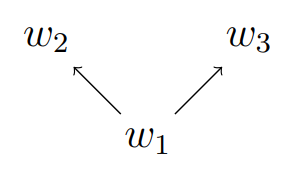
\includegraphics[width=0.15\textwidth]{hw05_1.png}
    \end{center}
    \item (1 балл) Допишите указание истинности переменных в следующей шкале Крипке так,
    чтобы она опровергала формулу $(\overline{p} \rightarrow q \lor r) \rightarrow (\overline{p} \rightarrow q) \lor (\overline{p} \rightarrow r)$:
    \begin{center}
        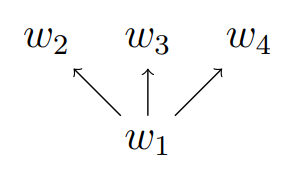
\includegraphics[width=0.15\textwidth]{hw05_2.png}
    \end{center}
    \item Постройте шкалы Крипке, опровергающие следующие формулы:
    \begin{itemize}
        \item[(a)] (1 балл) $(p \rightarrow q) \rightarrow \overline{p} \lor q$
        \item[(b)] (2 балл) $((p \rightarrow q) \rightarrow p) \rightarrow p$
    \end{itemize}
\end{enumerate}
\clearpage

  % \section{Алгебраические теории и логика первого порядка}
\begin{enumerate}
    \item (1б.) Опишите двухсортную сигнатуру и теорию коммутативных колец с единицей и модулей над ними.
    \begin{solution}
        $M$ -- модуль, $A$ -- коммутативное кольцо.
        \begin{eqnarray}
            &\Sigma = \langle\{A, M\}, \{*:A \times A \rightarrow A, +:A \times A \rightarrow A, e: A\}\rangle \\
            &(a*b)*m = a*(b*m), \quad \forall a, b \in A, m \in M \\
            &e*m = m, \quad m \in M \\
            &(a+b)*m = a*m+b*m, \quad \forall a, b \in A, m \in M \\
            &a*(m+n) = a*m+a*n, \quad \forall a \in A, m, n \in M
        \end{eqnarray}
    \end{solution}
    \item Выразите следующие свойства в логике первого порядка (запишите их в виде формул):
    \begin{itemize}
        \item[(a)] (1б.) ”Существует ровно два элемента, удовлетворяющих $P(x)$”
        \begin{solution}
            Придумал два решения:
            \begin{eqnarray}
                \exists x. \exists y. \forall z. \overline{(x=y)} \land \overline{(x=z)} \land \overline{(y=z)} \land P(x) \land P(y) \land \overline{P(z)} \\
                \exists x. \exists y. P(x) \land P(y) \land \overline{(x=y)} \land \forall z. P(z) \rightarrow (z = x \lor z = y)
            \end{eqnarray}
        \end{solution}
        \item[(b)] (1б.) ”Существует не менее двух элементов, удовлетворяющих $P(x)$”.
        \begin{solution}
            \begin{equation}
                \exists x. \exists y. P(x) \land P(y) \land \overline{(x=y)} \land \exists z. P(z) \land \overline{(z=x)} \land \overline{(z=y)}
            \end{equation}
        \end{solution}
        \item[(c)] (1б.) ”Существует по крайней мере один, но не более двух элементов, удовлетворяющих $P(x)$”
        \begin{solution}
            По сути это означает, что существует либо ровно 1, либо ровно 2 (пункт а), поэтому
            \begin{equation}
                \exists a(P(a) \land \forall b. P(b) \rightarrow (b = a)) \lor \exists x. \exists y. P(x) \land P(y) \land \overline{(x=y)} \land \forall z. P(z) \rightarrow (z = x \lor z = y)
            \end{equation}
        \end{solution}
        \item[(d)] (1б.) ”Существует не более одного элемента, удовлетворяющего $P(x)$”
        \begin{solution}
            По сути это означает, что существует либо ровно 0, либо ровно 1, поэтому
            \begin{equation}
                \forall c(\overline{P(c)}) \lor \exists a(P(a) \land \forall b. P(b) \rightarrow (b = a))
            \end{equation}
        \end{solution}
    \end{itemize}
    \item В стандартной интерпретации языка элементарной арифметики выразите следующие свойства:
    \begin{itemize}
        \item[(a)] (1б.) $q$ есть частное от деления $a$ на $b$;
        \begin{solution}
            Здесь и далее пользуюсь тем, что наша модель это $(\mathbb{R}, =, +, \cdot, 0, 1)$. Также удобно ввести порядок:
            \begin{equation}
                a \leq b \leftrightarrow \exists x. b = a + x \cdot x
            \end{equation}
            Дальше не очень понятно, что именно имеется в виду. Если имеется в виду $a/b = q$, то подойдет предикат $P(a,b,q)$
            \begin{equation}
                \exists q. \overline{(b=0)} \land q \cdot b = a
            \end{equation}
        \end{solution}
        \item[(b)] (1б.) $r$ есть остаток от деления $a$ на $b$;
        \item[(c)] (1б.) $s$ есть НОД $a$ и $b$;
        \item[(d)] (1б.) $t$ есть НОК $a$ и $b$;
        \item[(e)] (1б.) $a$ и $b$ взаимно просты;
        \item[(f)] (1б.) $u$ является степенью тройки.
    \end{itemize}
    Для сокращения записи пользуйтесь полученными ранее предикатами, введя для них вспомогательные символы.
    
\end{enumerate}
\clearpage

  \section{Практика 7}
\begin{enumerate}
    \item (1 балл) Покажите, что формула из лекции является общезначимой:
    $$(\exists x\varphi(x) \rightarrow \forall x\psi(x)) \rightarrow \forall x. \varphi(x) \rightarrow \psi(x)$$
    \item Покажите, что следующие формулы не являются общезначимыми (приведите контрпример — интерпретацию и значения переменных, как на лекции):
    \begin{itemize}
        \item[(a)] (0,5 балла) $\forall x\varphi \lor \psi \leftrightarrow \forall x. \varphi \lor \psi$
        \item[(b)] (0,5 балла) $\exists x\varphi \land \psi \leftrightarrow \exists x. \varphi \land \psi$
        \item[(c)] (0,5 балла) $\forall x\varphi \rightarrow \psi \leftrightarrow \exists x. \varphi \rightarrow \psi$
        \item[(d)] (0,5 балла) $\exists x\varphi \rightarrow \psi \leftrightarrow \forall x. \varphi \rightarrow \psi$
        \item[(e)] (0,5 балла) $\varphi \rightarrow \forall x\psi \leftrightarrow \forall x. \varphi \rightarrow \psi$
        \item[(f)] (0,5 балла) $\varphi \rightarrow \exists x\psi \leftrightarrow \exists x. \varphi \rightarrow \psi$
    \end{itemize}
    \item Постройте ПНФ формул и сколемизируйте результат до $\Pi_1$:
    \begin{itemize}
        \item[(a)] (1 балл) $\exists x\forall y P(x, y) \lor \exists x\forall y Q(x, y)$
        \begin{solution}
            \begin{align*}
                &\exists x\forall y P(x, y) \lor \exists x\forall y Q(x, y) \\
                &\exists x . \forall y P(x, y) \lor \forall y Q(x, y) \\
                &\exists x . \forall y P(x, y) \lor \forall z Q(x, z) \\
                &\exists x . \forall y. P(x, y) \lor \forall z Q(x, z) \\
                &\exists x . \forall y. \forall z . P(x, y) \lor Q(x, z) \\
                &\forall y. \forall z . P(x, y) \lor Q(x, z)
            \end{align*}
        \end{solution}
        \item[(b)] (1 балл) $\exists x\forall y P(x, y) \rightarrow \exists x\forall y Q(x, y)$
        \item[(c)] (2 балла) $\exists x. \forall y P(y) \rightarrow \overline{\exists z S(z)} \land \exists y Q(x, y)$
    \end{itemize}
\end{enumerate}
\clearpage


\end{document}
